% Options for packages loaded elsewhere
\PassOptionsToPackage{unicode}{hyperref}
\PassOptionsToPackage{hyphens}{url}
%
\documentclass[
]{book}
\usepackage{lmodern}
\usepackage{amssymb,amsmath}
\usepackage{ifxetex,ifluatex}
\ifnum 0\ifxetex 1\fi\ifluatex 1\fi=0 % if pdftex
  \usepackage[T1]{fontenc}
  \usepackage[utf8]{inputenc}
  \usepackage{textcomp} % provide euro and other symbols
\else % if luatex or xetex
  \usepackage{unicode-math}
  \defaultfontfeatures{Scale=MatchLowercase}
  \defaultfontfeatures[\rmfamily]{Ligatures=TeX,Scale=1}
\fi
% Use upquote if available, for straight quotes in verbatim environments
\IfFileExists{upquote.sty}{\usepackage{upquote}}{}
\IfFileExists{microtype.sty}{% use microtype if available
  \usepackage[]{microtype}
  \UseMicrotypeSet[protrusion]{basicmath} % disable protrusion for tt fonts
}{}
\makeatletter
\@ifundefined{KOMAClassName}{% if non-KOMA class
  \IfFileExists{parskip.sty}{%
    \usepackage{parskip}
  }{% else
    \setlength{\parindent}{0pt}
    \setlength{\parskip}{6pt plus 2pt minus 1pt}}
}{% if KOMA class
  \KOMAoptions{parskip=half}}
\makeatother
\usepackage{xcolor}
\IfFileExists{xurl.sty}{\usepackage{xurl}}{} % add URL line breaks if available
\IfFileExists{bookmark.sty}{\usepackage{bookmark}}{\usepackage{hyperref}}
\hypersetup{
  pdftitle={R como herramienta de escritura académico-científica con visualización estática y dinámica},
  pdfauthor={Alexander Andrade},
  hidelinks,
  pdfcreator={LaTeX via pandoc}}
\urlstyle{same} % disable monospaced font for URLs
\usepackage{color}
\usepackage{fancyvrb}
\newcommand{\VerbBar}{|}
\newcommand{\VERB}{\Verb[commandchars=\\\{\}]}
\DefineVerbatimEnvironment{Highlighting}{Verbatim}{commandchars=\\\{\}}
% Add ',fontsize=\small' for more characters per line
\usepackage{framed}
\definecolor{shadecolor}{RGB}{248,248,248}
\newenvironment{Shaded}{\begin{snugshade}}{\end{snugshade}}
\newcommand{\AlertTok}[1]{\textcolor[rgb]{0.94,0.16,0.16}{#1}}
\newcommand{\AnnotationTok}[1]{\textcolor[rgb]{0.56,0.35,0.01}{\textbf{\textit{#1}}}}
\newcommand{\AttributeTok}[1]{\textcolor[rgb]{0.77,0.63,0.00}{#1}}
\newcommand{\BaseNTok}[1]{\textcolor[rgb]{0.00,0.00,0.81}{#1}}
\newcommand{\BuiltInTok}[1]{#1}
\newcommand{\CharTok}[1]{\textcolor[rgb]{0.31,0.60,0.02}{#1}}
\newcommand{\CommentTok}[1]{\textcolor[rgb]{0.56,0.35,0.01}{\textit{#1}}}
\newcommand{\CommentVarTok}[1]{\textcolor[rgb]{0.56,0.35,0.01}{\textbf{\textit{#1}}}}
\newcommand{\ConstantTok}[1]{\textcolor[rgb]{0.00,0.00,0.00}{#1}}
\newcommand{\ControlFlowTok}[1]{\textcolor[rgb]{0.13,0.29,0.53}{\textbf{#1}}}
\newcommand{\DataTypeTok}[1]{\textcolor[rgb]{0.13,0.29,0.53}{#1}}
\newcommand{\DecValTok}[1]{\textcolor[rgb]{0.00,0.00,0.81}{#1}}
\newcommand{\DocumentationTok}[1]{\textcolor[rgb]{0.56,0.35,0.01}{\textbf{\textit{#1}}}}
\newcommand{\ErrorTok}[1]{\textcolor[rgb]{0.64,0.00,0.00}{\textbf{#1}}}
\newcommand{\ExtensionTok}[1]{#1}
\newcommand{\FloatTok}[1]{\textcolor[rgb]{0.00,0.00,0.81}{#1}}
\newcommand{\FunctionTok}[1]{\textcolor[rgb]{0.00,0.00,0.00}{#1}}
\newcommand{\ImportTok}[1]{#1}
\newcommand{\InformationTok}[1]{\textcolor[rgb]{0.56,0.35,0.01}{\textbf{\textit{#1}}}}
\newcommand{\KeywordTok}[1]{\textcolor[rgb]{0.13,0.29,0.53}{\textbf{#1}}}
\newcommand{\NormalTok}[1]{#1}
\newcommand{\OperatorTok}[1]{\textcolor[rgb]{0.81,0.36,0.00}{\textbf{#1}}}
\newcommand{\OtherTok}[1]{\textcolor[rgb]{0.56,0.35,0.01}{#1}}
\newcommand{\PreprocessorTok}[1]{\textcolor[rgb]{0.56,0.35,0.01}{\textit{#1}}}
\newcommand{\RegionMarkerTok}[1]{#1}
\newcommand{\SpecialCharTok}[1]{\textcolor[rgb]{0.00,0.00,0.00}{#1}}
\newcommand{\SpecialStringTok}[1]{\textcolor[rgb]{0.31,0.60,0.02}{#1}}
\newcommand{\StringTok}[1]{\textcolor[rgb]{0.31,0.60,0.02}{#1}}
\newcommand{\VariableTok}[1]{\textcolor[rgb]{0.00,0.00,0.00}{#1}}
\newcommand{\VerbatimStringTok}[1]{\textcolor[rgb]{0.31,0.60,0.02}{#1}}
\newcommand{\WarningTok}[1]{\textcolor[rgb]{0.56,0.35,0.01}{\textbf{\textit{#1}}}}
\usepackage{longtable,booktabs}
% Correct order of tables after \paragraph or \subparagraph
\usepackage{etoolbox}
\makeatletter
\patchcmd\longtable{\par}{\if@noskipsec\mbox{}\fi\par}{}{}
\makeatother
% Allow footnotes in longtable head/foot
\IfFileExists{footnotehyper.sty}{\usepackage{footnotehyper}}{\usepackage{footnote}}
\makesavenoteenv{longtable}
\usepackage{graphicx,grffile}
\makeatletter
\def\maxwidth{\ifdim\Gin@nat@width>\linewidth\linewidth\else\Gin@nat@width\fi}
\def\maxheight{\ifdim\Gin@nat@height>\textheight\textheight\else\Gin@nat@height\fi}
\makeatother
% Scale images if necessary, so that they will not overflow the page
% margins by default, and it is still possible to overwrite the defaults
% using explicit options in \includegraphics[width, height, ...]{}
\setkeys{Gin}{width=\maxwidth,height=\maxheight,keepaspectratio}
% Set default figure placement to htbp
\makeatletter
\def\fps@figure{htbp}
\makeatother
\setlength{\emergencystretch}{3em} % prevent overfull lines
\providecommand{\tightlist}{%
  \setlength{\itemsep}{0pt}\setlength{\parskip}{0pt}}
\setcounter{secnumdepth}{5}
\usepackage{booktabs}
\usepackage[]{natbib}
\bibliographystyle{apalike}

\title{R como herramienta de escritura académico-científica con visualización estática y dinámica}
\author{Alexander Andrade}
\date{2020-02-29}

\begin{document}
\frontmatter
\maketitle

{
\setcounter{tocdepth}{1}
\tableofcontents
}
\mainmatter
\hypertarget{resumen}{%
\chapter{Resumen}\label{resumen}}

R es un lenguaje de programación estadística, que permite: importar, gestionar, analizar y presentar información (datos), con un alto nivel de reproducibilidad. Consolidándose así, como el software ideal en: estadística, machine learning, ciencia de datos, etc.

En el taller denominado \emph{R como herramienta de escritura académico-científica con visualización estática y dinámica}, se estudian las ventajas que ofrece el paquete \texttt{rmarkdown}, el cual permite generar reportes estáticos y dinámicos, con el fin de divulgar tanto los resultados de un estudio, como su metodología y el código utilizado.

Particularmente, el taller se enfoca en la creación de libros académico-científicos (en formato HTML, EPUB y PDF) mediante el paquete \texttt{bookdown}, mismo que puede entenderse como una extensión de \texttt{rmarkdown}.

Al finalizar el taller, los asistentes serán capaces de:

\begin{itemize}
\tightlist
\item
  Entender de manera global, el funcionamiento de \texttt{rmarkdown}, su sintaxis y sus principales características.
\item
  Construir libros digitales mediante el paquete \texttt{bookdown} (similares al libro que se está visualizando en este momento).
\item
  Conocer la diferencia entre visualización estática y dinámica.
\item
  Incorporar las bondades de \texttt{bookdown} en la divulgación científica.
\end{itemize}

\hypertarget{bibliografuxeda-buxe1sica}{%
\section*{Bibliografía básica}\label{bibliografuxeda-buxe1sica}}
\addcontentsline{toc}{section}{Bibliografía básica}

\textbf{Libros:}

\begin{itemize}
\tightlist
\item
  \emph{Bookdown: Authoring Books and Technical Documents with R Markdown} \citep{xie2016bookdown}
\item
  \emph{R markdown: The definitive guide} \citep{xie2018r}
\item
  \emph{Dynamic Documents with R and knitr} \citep{xie2015}
\end{itemize}

\textbf{Paquetes:}

\begin{itemize}
\tightlist
\item
  \emph{Bookdown} \citep{R-bookdown}
\item
  \emph{Rmarkdown} \citep{R-rmarkdown}
\end{itemize}

\hypertarget{requi}{%
\chapter{Requisitos para el taller}\label{requi}}

\hypertarget{conocimiento-previo-recomendado}{%
\section{Conocimiento previo (Recomendado)}\label{conocimiento-previo-recomendado}}

\begin{itemize}
\tightlist
\item
  Entendimiento básico de R y RStudio.
\item
  Nivel básico de \texttt{rmarkdown}
\end{itemize}

\textbf{¿Qué ocurre si nunca he trabajado con R, Rstudio o rmarkdown?}

Previo a este taller, se impartirán charlas y talleres en los siguientes temas:

\begin{itemize}
\tightlist
\item
  R/RStudio
\item
  Rmarkdown
\item
  R shiny
\end{itemize}

Los cuales brindarán un importante background teórico-práctico sobre R.

\hypertarget{software}{%
\section{Software}\label{software}}

\hypertarget{recursos-indispensables}{%
\subsection{Recursos indispensables}\label{recursos-indispensables}}

\begin{enumerate}
\def\labelenumi{\arabic{enumi}.}
\item
  Lenguaje de programación estadística \textbf{R:} \url{https://cran.r-project.org/}
\item
  Interfaz de desarrollo integrado \textbf{RStudio:} \url{https://rstudio.com/products/rstudio/download/}
\item
  \textbf{MiKTeX:} \url{https://miktex.org/download}
\end{enumerate}

\textbf{\emph{Nota:}} Se recomienda que la instalación de los recursos previamente mencionados, se realice en el orden en el que fueron enumerados.

\hypertarget{recursos-recomendados}{%
\subsection{Recursos recomendados}\label{recursos-recomendados}}

\begin{enumerate}
\def\labelenumi{\arabic{enumi}.}
\item
  Lector de PDF
\item
  Lector de EPUB
\end{enumerate}

\textbf{\emph{Nota:}} El lector de archivos PDF y archivos EPUB queda a disposición de los asistentes. Una posible opción es \href{https://fbreader.org/}{FDReader} (recomendado).

\hypertarget{paquetes}{%
\subsection{Paquetes}\label{paquetes}}

\begin{enumerate}
\def\labelenumi{\arabic{enumi}.}
\tightlist
\item
  \texttt{tidyverse}
\end{enumerate}

\begin{Shaded}
\begin{Highlighting}[]
\KeywordTok{install.packages}\NormalTok{(}\StringTok{"tidyverse"}\NormalTok{)}
\end{Highlighting}
\end{Shaded}

\begin{enumerate}
\def\labelenumi{\arabic{enumi}.}
\setcounter{enumi}{1}
\tightlist
\item
  \texttt{bookdown}
\end{enumerate}

\begin{Shaded}
\begin{Highlighting}[]
\KeywordTok{install.packages}\NormalTok{(}\StringTok{"bookdown"}\NormalTok{)}
\end{Highlighting}
\end{Shaded}

\begin{enumerate}
\def\labelenumi{\arabic{enumi}.}
\setcounter{enumi}{2}
\tightlist
\item
  \texttt{shiny}
\end{enumerate}

\begin{Shaded}
\begin{Highlighting}[]
\KeywordTok{install.packages}\NormalTok{(}\StringTok{"shiny"}\NormalTok{)}
\end{Highlighting}
\end{Shaded}

\begin{enumerate}
\def\labelenumi{\arabic{enumi}.}
\setcounter{enumi}{3}
\tightlist
\item
  \texttt{knitr}
\end{enumerate}

\begin{Shaded}
\begin{Highlighting}[]
\KeywordTok{install.packages}\NormalTok{(}\StringTok{"knitr"}\NormalTok{)}
\end{Highlighting}
\end{Shaded}

\begin{enumerate}
\def\labelenumi{\arabic{enumi}.}
\setcounter{enumi}{4}
\tightlist
\item
  \texttt{DT}
\end{enumerate}

\begin{Shaded}
\begin{Highlighting}[]
\KeywordTok{install.packages}\NormalTok{(}\StringTok{"DT"}\NormalTok{)}
\end{Highlighting}
\end{Shaded}

\begin{enumerate}
\def\labelenumi{\arabic{enumi}.}
\setcounter{enumi}{5}
\tightlist
\item
  \texttt{plotly}
\end{enumerate}

\begin{Shaded}
\begin{Highlighting}[]
\KeywordTok{install.packages}\NormalTok{(}\StringTok{"plotly"}\NormalTok{)}
\end{Highlighting}
\end{Shaded}

\begin{enumerate}
\def\labelenumi{\arabic{enumi}.}
\setcounter{enumi}{6}
\tightlist
\item
  \texttt{tinytex}
\end{enumerate}

\begin{Shaded}
\begin{Highlighting}[]
\KeywordTok{install.packages}\NormalTok{(}\StringTok{"tinytex"}\NormalTok{)}
\NormalTok{tinytex}\OperatorTok{::}\KeywordTok{install_tinytex}\NormalTok{()}
\end{Highlighting}
\end{Shaded}

\begin{enumerate}
\def\labelenumi{\arabic{enumi}.}
\setcounter{enumi}{7}
\tightlist
\item
  \texttt{phantomjs}
\end{enumerate}

\begin{Shaded}
\begin{Highlighting}[]
\KeywordTok{install.packages}\NormalTok{(}\StringTok{"webshot"}\NormalTok{)}
\NormalTok{webshot}\OperatorTok{::}\KeywordTok{install_phantomjs}\NormalTok{()}
\end{Highlighting}
\end{Shaded}

\hypertarget{intro}{%
\chapter{Introducción}\label{intro}}

La reproducibilidad es sumamente importante en investigación científica y en el proceso de enseñanza-aprendizaje, principalmente cuando se está enseñando (o aprendiendo) un lenguaje de programación. En tal contexto, el paquete \texttt{bookdown} permite compartir el código y los resultados de un experimento en forma de libros virtuales, ayudando al investigador o docente, a enfocarse en el aspecto científico y facilitando el proceso de redacción.

\textbf{Principales ventajas de \texttt{bookdown}}

\begin{itemize}
\tightlist
\item
  Reproducibilidad de la investigación.
\item
  Existe una gran cantidad de temas o templates que permiten crear libros virtuales estéticamente agradables.
\item
  La optimización del paquete con la interfaz de RStudio logra un vínculo amigable para el usuario.
\item
  La estructura de la herramienta resalta las características propias de la redacción científica.
\item
  Los formatos de salida del libro automáticamente contemplan: HTML, PDF, EPUB.
\item
  En formato HTML es posible presentar los resultados de forma dinámica, es decir, el lector podrá interactuar con la información que se comparte en el libro.
\item
  Es posible crear quiz interactivos para el lector, de tal manera que su aprendizaje se vea reforzado mediante la práctica.
\end{itemize}

\hypertarget{visualizacion}{%
\chapter{Visualización Estática y Dinámica}\label{visualizacion}}

Como se mencionó en el capítulo anterior, una de las ventajas de \texttt{bookdown} es la visualización dinámica de resultados. En este apartado se presentan varios ejemplos con la intención de resaltar las bondades de la visualización dinámica, sobre la visualización estática. Es importante tener en claro que la visualización dinámica de resultados es posible únicamente en la versión HTML del libro digital.

\hypertarget{visualizaciuxf3n-estuxe1tica}{%
\section{Visualización Estática}\label{visualizaciuxf3n-estuxe1tica}}

\hypertarget{ejemplo-1}{%
\subsection{Ejemplo 1}\label{ejemplo-1}}

A continuación se presenta una tabla con las diez primeras observaciones del dataset \texttt{Iris}. Este conjunto de datos está conformado por medidas de ciertas características físicas de pétalos y sépalos sobre 150 plantas, tomando en cuenta tres especies: Setosa, Versicolor y Virginica.

\begin{Shaded}
\begin{Highlighting}[]
\NormalTok{knitr}\OperatorTok{::}\KeywordTok{kable}\NormalTok{(}\KeywordTok{head}\NormalTok{(iris, }\DecValTok{10}\NormalTok{))}
\end{Highlighting}
\end{Shaded}

\begin{tabular}{r|r|r|r|l}
\hline
Sepal.Length & Sepal.Width & Petal.Length & Petal.Width & Species\\
\hline
5.1 & 3.5 & 1.4 & 0.2 & setosa\\
\hline
4.9 & 3.0 & 1.4 & 0.2 & setosa\\
\hline
4.7 & 3.2 & 1.3 & 0.2 & setosa\\
\hline
4.6 & 3.1 & 1.5 & 0.2 & setosa\\
\hline
5.0 & 3.6 & 1.4 & 0.2 & setosa\\
\hline
5.4 & 3.9 & 1.7 & 0.4 & setosa\\
\hline
4.6 & 3.4 & 1.4 & 0.3 & setosa\\
\hline
5.0 & 3.4 & 1.5 & 0.2 & setosa\\
\hline
4.4 & 2.9 & 1.4 & 0.2 & setosa\\
\hline
4.9 & 3.1 & 1.5 & 0.1 & setosa\\
\hline
\end{tabular}

Aún cuando la tabla es estéticamente agradable, únicamente se observa una cierta cantidad de datos, los cuales no siguen ningún orden específico, y además, no es posible filtrar la información según ciertos parámetros de interés.

\hypertarget{ejm2}{%
\subsection{Ejemplo 2}\label{ejm2}}

La información del dataset \texttt{Iris} se resume en un diagrama de caja (boxplot), el cual compara la longitud del sépalo de las plantas, tomando en cuenta las tres especies bajo estudio.

\begin{Shaded}
\begin{Highlighting}[]
\KeywordTok{library}\NormalTok{(tidyverse)}

\NormalTok{iris }\OperatorTok\StringTok{ }
\StringTok{  }\KeywordTok{ggplot}\NormalTok{(}\KeywordTok{aes}\NormalTok{(Species, Sepal.Length, }\DataTypeTok{fill =}\NormalTok{ Species)) }\OperatorTok{+}
\StringTok{  }\KeywordTok{geom_boxplot}\NormalTok{()}
\end{Highlighting}
\end{Shaded}

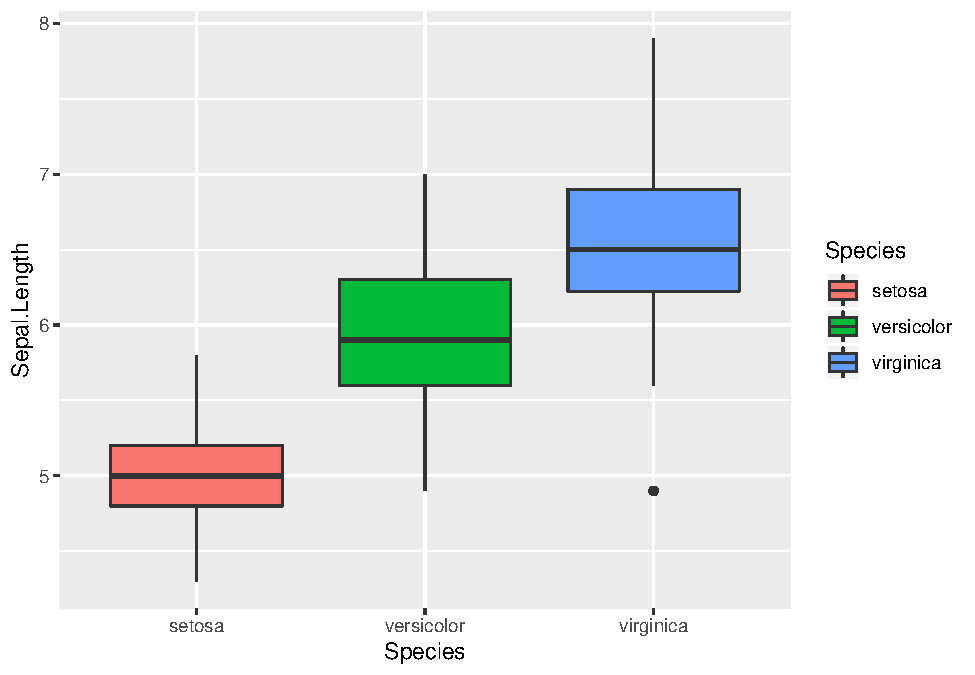
\includegraphics{flisol_bookdown_files/figure-latex/unnamed-chunk-10-1.pdf}

El boxplot es una herramienta visual muy importante y útil a la hora de comparar una variable medida en muestras de diferentes poblaciones. Si bien el gráfico nos presenta información relevante sobre los individuos (plantas), esta información puede aprovecharse de mejor manera con técnicas de visualización dinámica.

\hypertarget{visualizaciuxf3n-dinuxe1mica}{%
\section{Visualización Dinámica}\label{visualizaciuxf3n-dinuxe1mica}}

\hypertarget{ejemplo-3}{%
\subsection{Ejemplo 3}\label{ejemplo-3}}

Nuevamente se presenta el dataset \texttt{Iris}, pero ahora mediante una tabla dinámica. En este caso el lector puede interactuar con la tabla, realizando las siguientes acciones:

\begin{itemize}
\tightlist
\item
  Cambiar el número de observaciones que se muestran (\textbf{\emph{Show entries}}). Por defecto se pueden mostrar 10, 25, 50 o 100 observaciones. Este rango de valores se puede cambiar según las necesidades del investigador.
\item
  Buscar (\textbf{\emph{Search}}) un tipo de planta o un número en particular. Por ejemplo, el lector puede buscar la palabra ``\emph{virginica}'', de tal forma que se muestren únicamente las observaciones de esta especie.
\item
  Ordenar el dataset según una de las variables, de forma ascendente o descendente. Para ello, el lector simplemente debe dar clic en el nombre de la variable que se quiera ordenar.
\item
  Visualizar (\textbf{\emph{Previous}}) diferentes porciones del dataset.
\end{itemize}

\begin{Shaded}
\begin{Highlighting}[]
\NormalTok{DT}\OperatorTok{::}\KeywordTok{datatable}\NormalTok{(\{iris\})}
\end{Highlighting}
\end{Shaded}

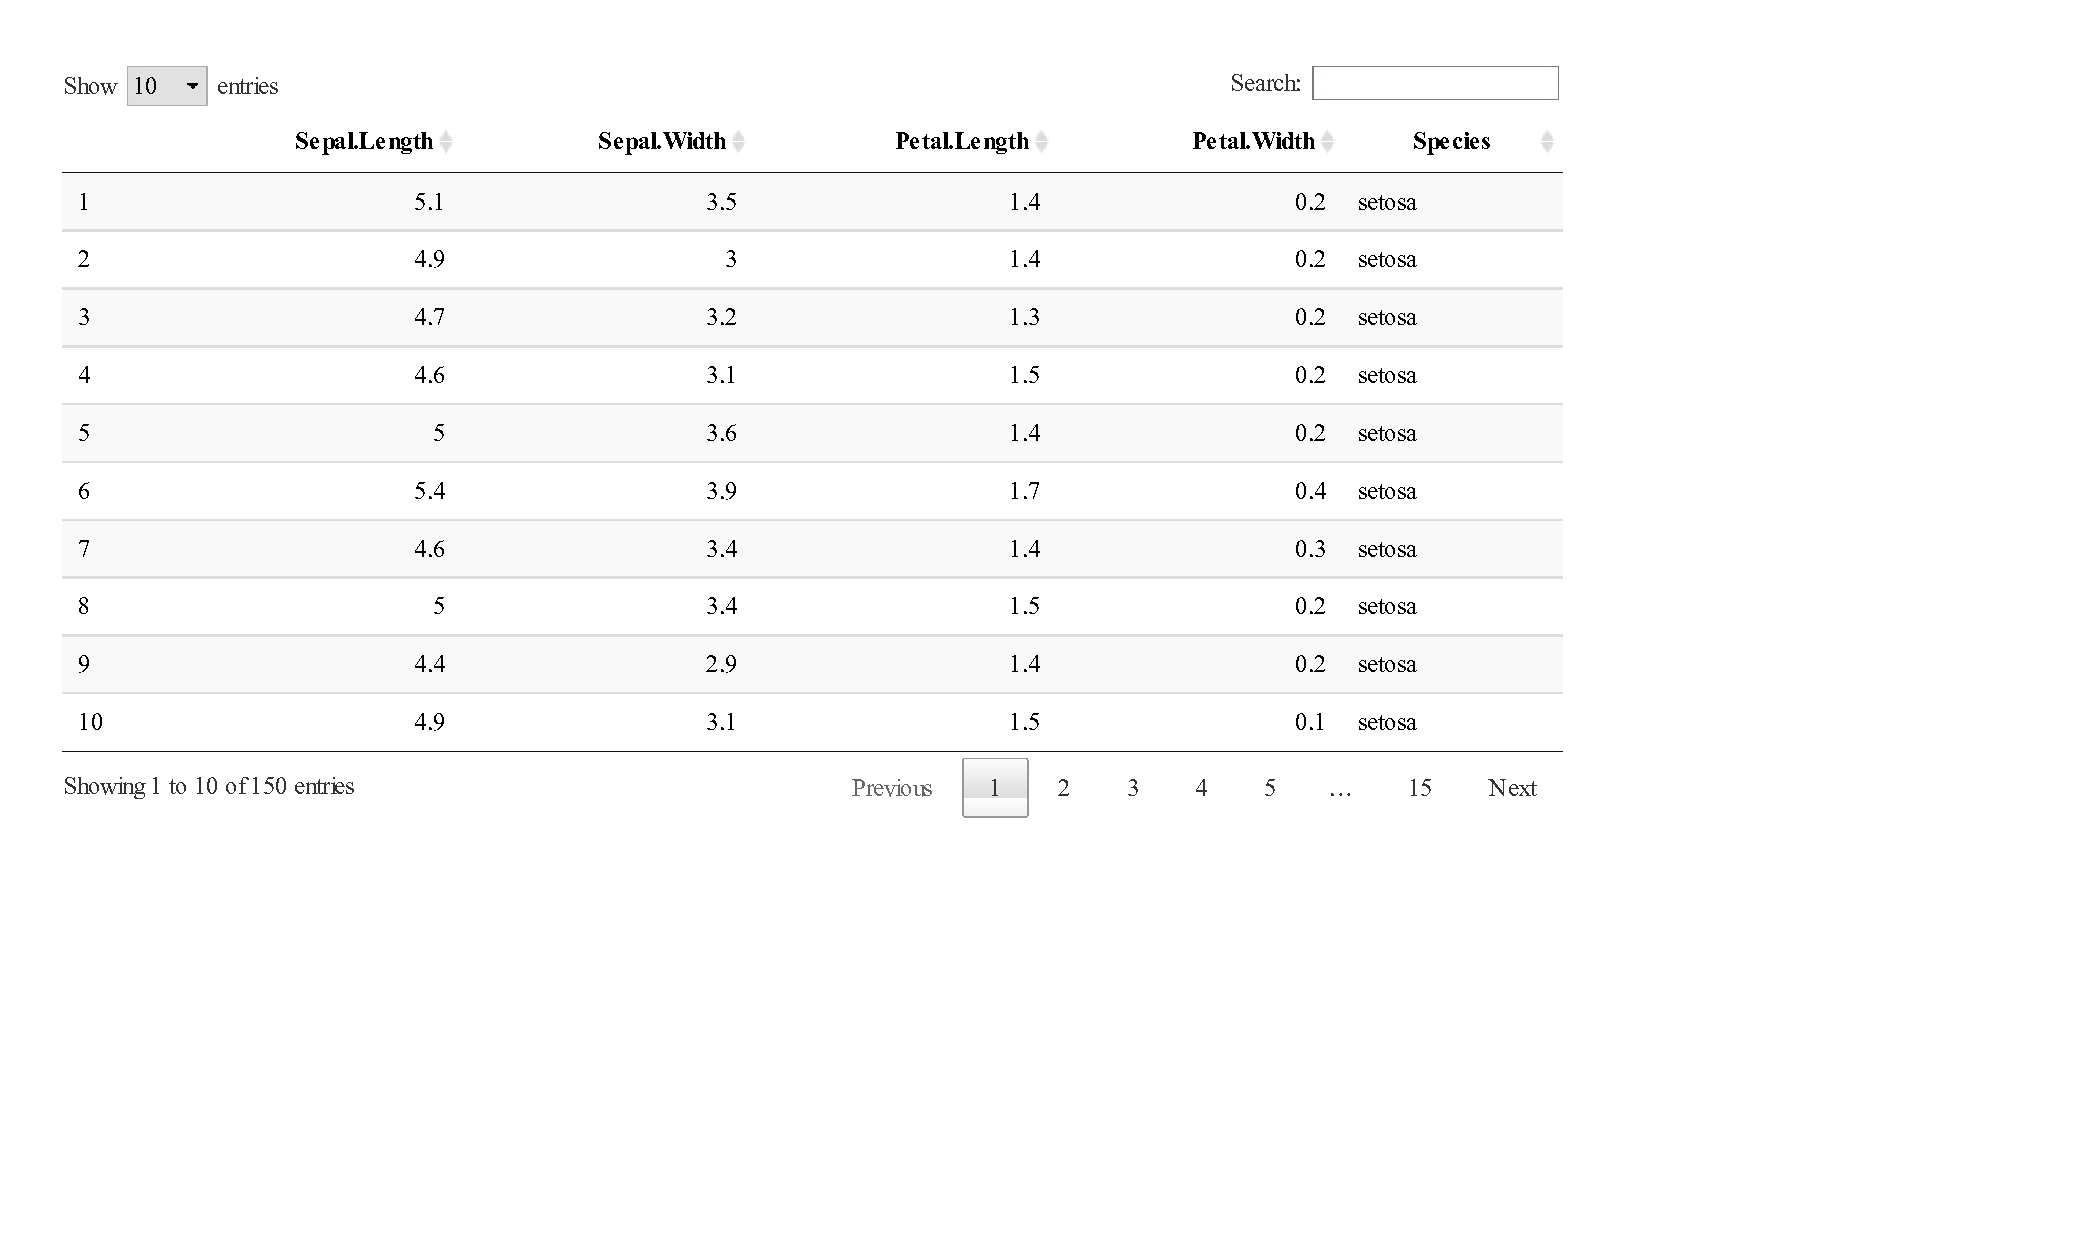
\includegraphics{flisol_bookdown_files/figure-latex/unnamed-chunk-11-1.pdf}

\hypertarget{ejm4}{%
\subsection{Ejemplo 4}\label{ejm4}}

En este ejemplo se presenta el mismo boxplot del \protect\hyperlink{ejm2}{Ejemplo 2}, en formato dinámico. En este gráfico, el lector puede realizar las siguientes acciones:

\begin{itemize}
\tightlist
\item
  Al pasar el puntero del mouse sobre el boxplot, es posible obtener información específica sobre los valores de: cuartiles, máximo, mínimo, datos atípicos.
\item
  En la parte superior del gráfico aparece una barra con las siguientes opciones: descargar el gráfico, realizar zoom, centrar la imagen, auto escalar, etc. El lector puede hacer uso de cualquiera de estas opciones sin preocuparse por afectar permanentemente el documento.
\item
  Al dar clic sobre una de las tres especies que se muestran en la leyenda (\textbf{\emph{Species}}), el lector podrá habilitar o deshabilitar cualquiera de los tres diagramas de caja que se muestran.
\end{itemize}

\begin{Shaded}
\begin{Highlighting}[]
\NormalTok{p <-}\StringTok{ }\NormalTok{iris }\OperatorTok\StringTok{ }
\StringTok{  }\KeywordTok{ggplot}\NormalTok{(}\KeywordTok{aes}\NormalTok{(Species, Sepal.Length, }\DataTypeTok{fill =}\NormalTok{ Species)) }\OperatorTok{+}
\StringTok{  }\KeywordTok{geom_boxplot}\NormalTok{()}

\NormalTok{plotly}\OperatorTok{::}\KeywordTok{ggplotly}\NormalTok{(p)}
\end{Highlighting}
\end{Shaded}


\includegraphics{flisol_bookdown_files/figure-latex/unnamed-chunk-12-1.pdf}

\hypertarget{ejemplo-5}{%
\subsection{Ejemplo 5}\label{ejemplo-5}}

Finalmente, se presenta otra forma de visualización dinámica del boxplot que hemos analizado en los ejemplos \protect\hyperlink{ejm2}{2} y \protect\hyperlink{ejm4}{4}, en dichos ejemplos se ha visualizado únicamente la variable longitud del sépalo (\emph{Sepal.Length}). A continuación, el lector podrá escoger la variable del dataset \texttt{Iris} que prefiera analizar.

\begin{Shaded}
\begin{Highlighting}[]
\NormalTok{knitr}\OperatorTok{::}\KeywordTok{include_app}\NormalTok{(}\StringTok{"https://vaashub.shinyapps.io/iris_boxplot/"}\NormalTok{, }
  \DataTypeTok{height =} \StringTok{"650px"}\NormalTok{)}
\end{Highlighting}
\end{Shaded}

\href{https://vaashub.shinyapps.io/iris_boxplot/}{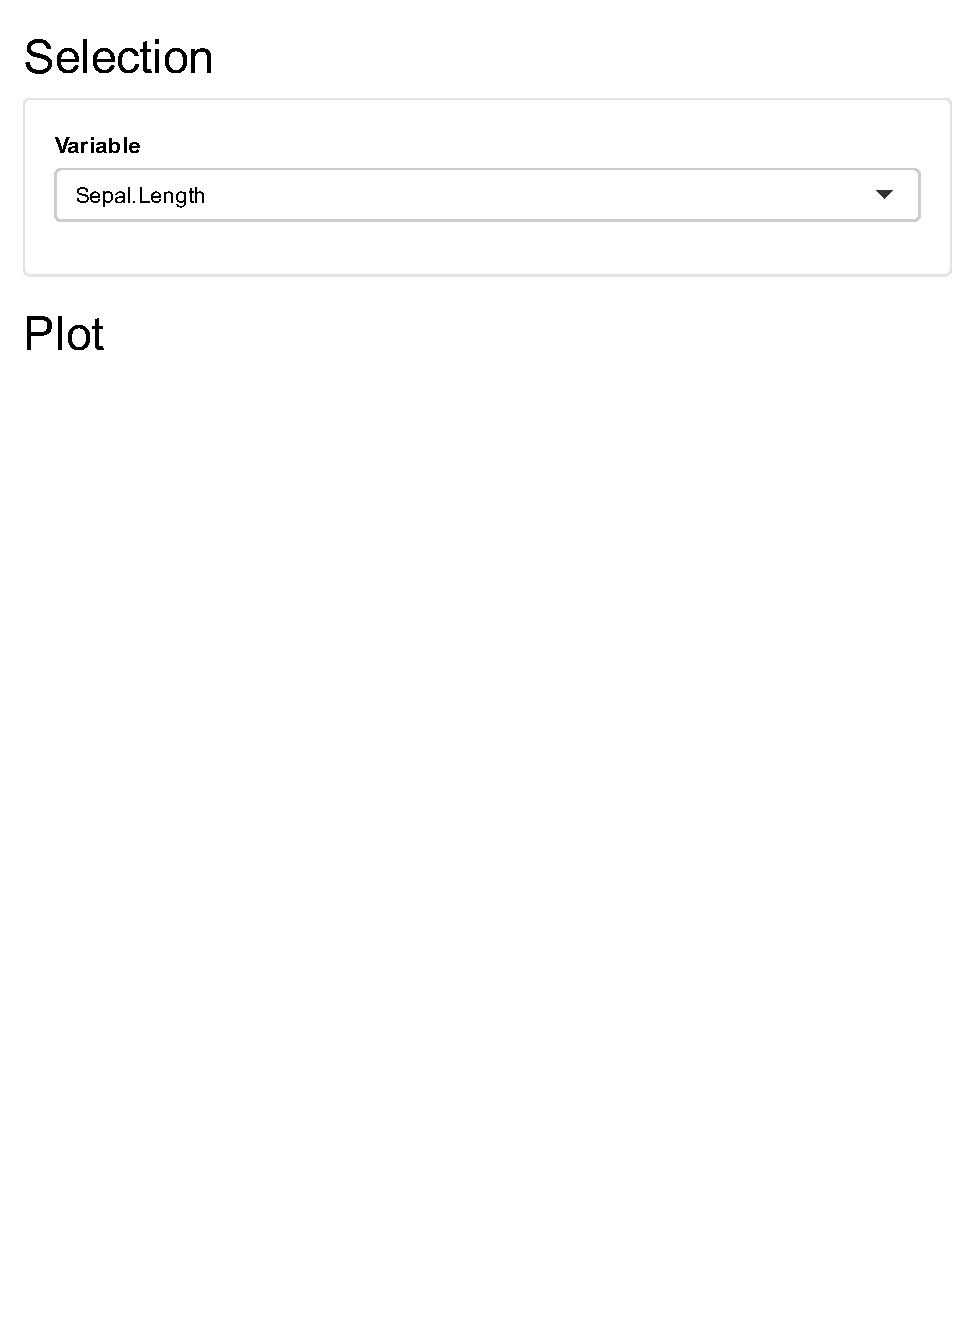
\includegraphics{flisol_bookdown_files/figure-latex/unnamed-chunk-13-1.pdf}}

\hypertarget{demuestra-lo-aprendido}{%
\chapter{Demuestra lo aprendido}\label{demuestra-lo-aprendido}}

\href{https://vaashub.shinyapps.io/quiz/}{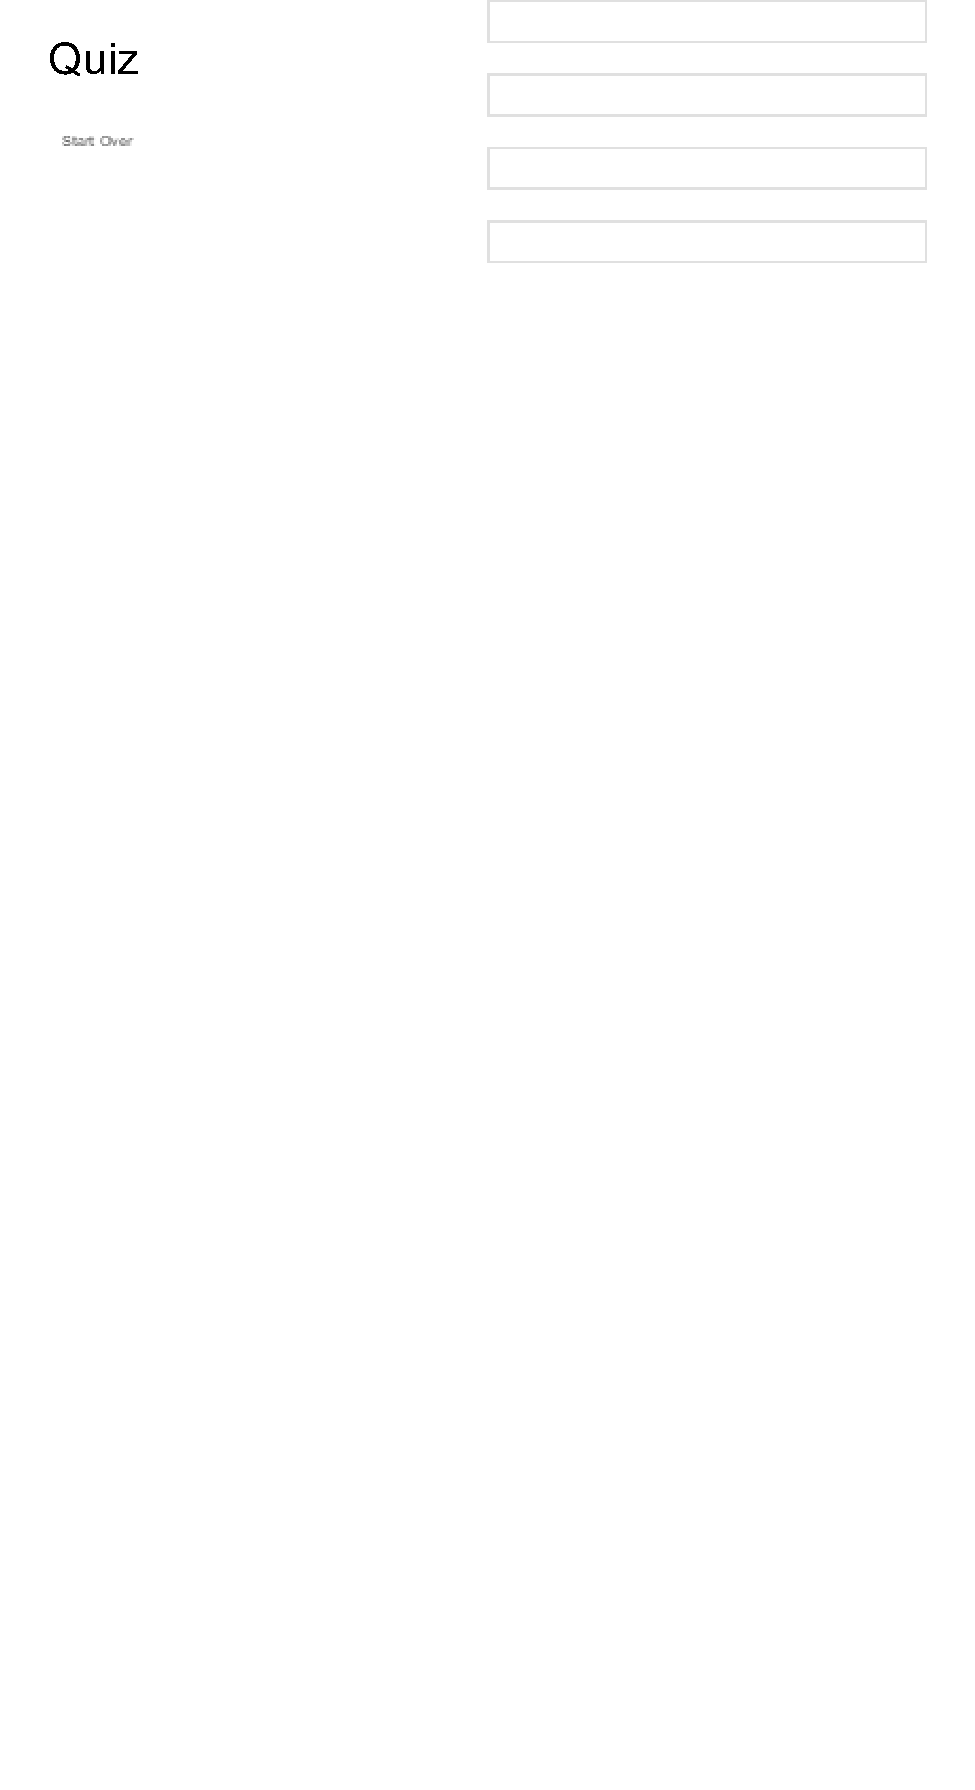
\includegraphics{flisol_bookdown_files/figure-latex/unnamed-chunk-14-1.pdf}}

\hypertarget{acerca-del-autor}{%
\chapter{Acerca del autor}\label{acerca-del-autor}}

\begin{flushleft}
\includegraphics[width=1\linewidth]{new} \end{flushleft}

\textbf{ALEXANDER ANDRADE}

Asesor Estadístico en \href{https://www.estadisticaparanoestadisticos.com}{Estadística para No Estadísticos}

\textbf{Estadística para No Estadísticos} brinda asesoría y tutoría estadística en:

\begin{itemize}
\tightlist
\item
  Data Science para: Instituciones, Empresas y Profesionales
\item
  Trabajos de Titulación (Pregrado y Posgrado)
\item
  Artículos Científicos (Papers)
\item
  Artículos de Revisión Bibliográfica mediante Minería de Texto
\end{itemize}

\textbf{¿Tienes dudas o comentarios?}

Contáctanos: \href{https://www.estadisticaparanoestadisticos.com}{www.estadisticaparanoestadisticos.com}

\backmatter
  \bibliography{book.bib,packages.bib}

\end{document}
